\documentclass[tikz,border=0pt]{standalone}
\usepackage[T1]{fontenc}
\usepackage[default,semibold]{sourcesanspro}
\usepackage{newtxsf}
\usepackage{amssymb}
\usepackage{tikz}
\usetikzlibrary{arrows.meta,positioning,calc,shapes.geometric,fit}

\definecolor{cA}{HTML}{0F766E}
\definecolor{cAbg}{HTML}{ECFDF5}
\definecolor{cGit}{HTML}{4338CA}
\definecolor{cGitbg}{HTML}{EEF2FF}
\definecolor{cDet}{HTML}{334155}
\definecolor{cDetbg}{HTML}{F1F5F9}
\definecolor{cB}{HTML}{B45309}
\definecolor{cBbg}{HTML}{FFFBEB}
\definecolor{cHum}{HTML}{BE123C}
\definecolor{cHumbg}{HTML}{FFF1F2}
\definecolor{ink}{HTML}{0F172A}
\definecolor{mid}{HTML}{64748B}
\definecolor{hair}{HTML}{CBD5E1}
\definecolor{band}{HTML}{1E2A55}

\newcommand{\zk}[1]{{\scriptsize\bfseries\color{mid}#1}}
\newcommand{\zh}[1]{{\small\bfseries\color{band}#1}}
\newcommand{\nt}[1]{{\scriptsize\bfseries #1}}
\newcommand{\nb}[1]{{\tiny #1}}
\newcommand{\an}[1]{{\tiny\color{mid}#1}}
\newcommand{\inv}[1]{{\tiny\bfseries\color{band}#1}}

\begin{document}
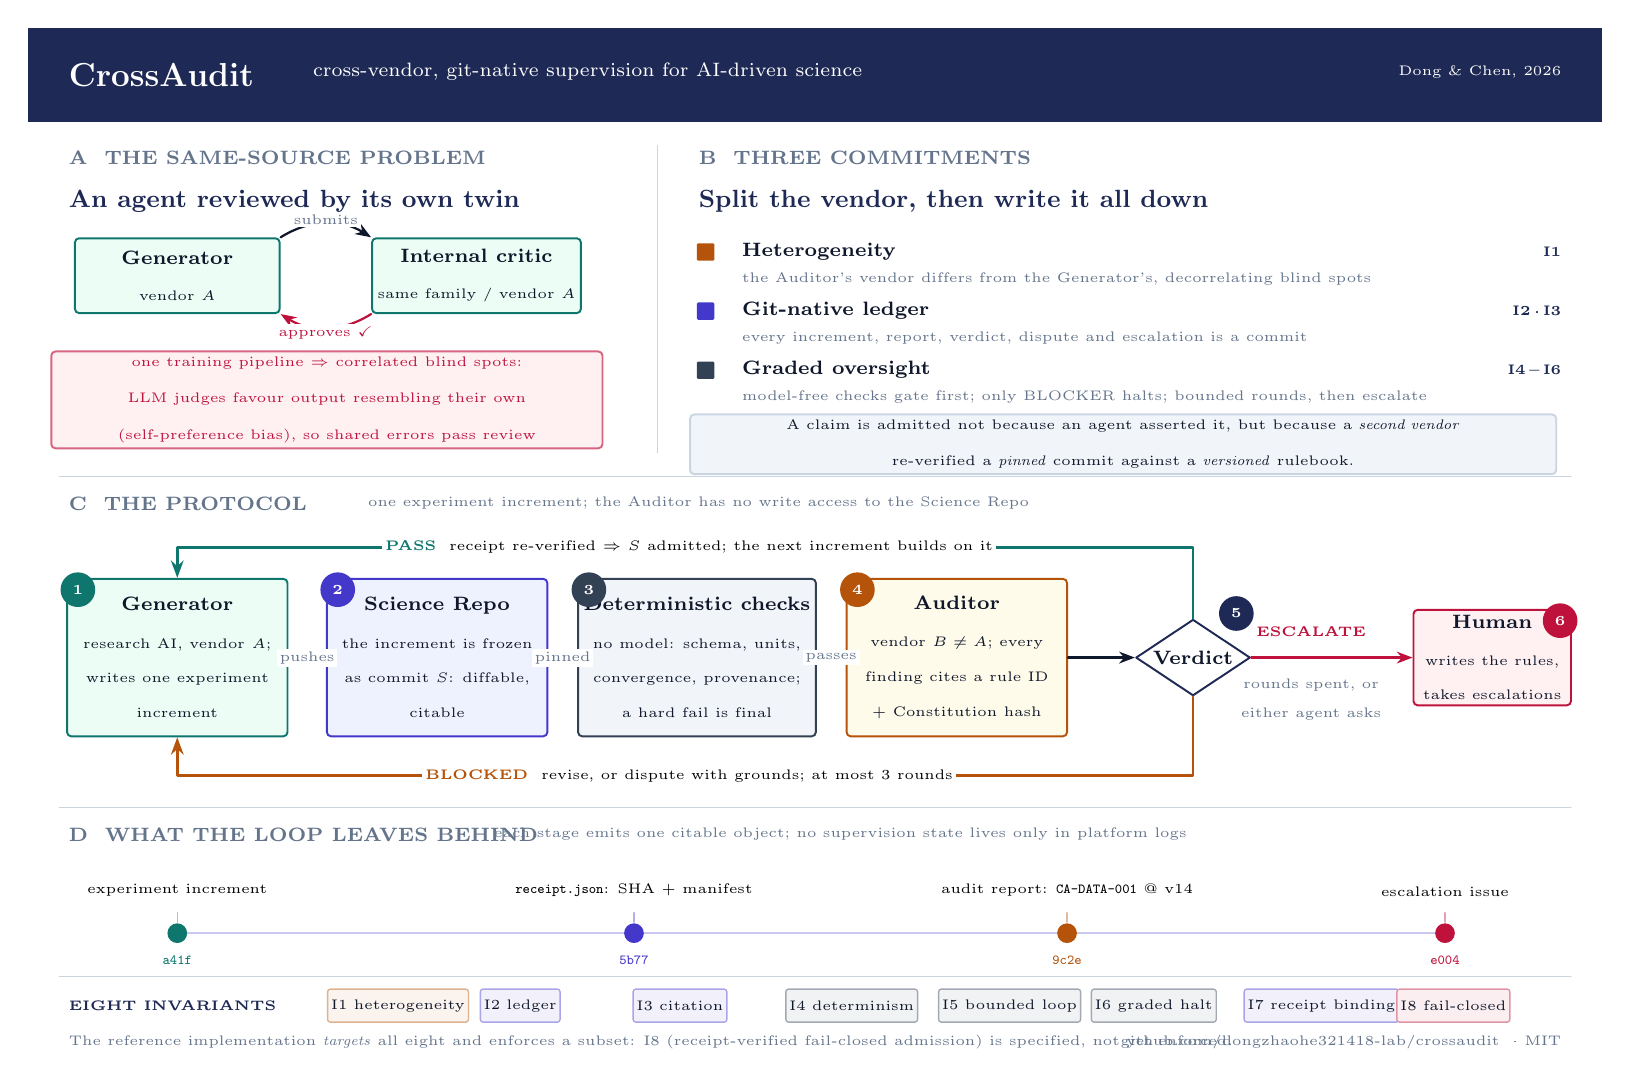
\begin{tikzpicture}[x=1mm,y=1mm,line join=round,line cap=round,
  every node/.append style={execute at begin node=\hyphenpenalty10000\exhyphenpenalty10000\relax}]
\tikzset{
  box/.style={rounded corners=1.5pt,line width=.7pt,align=center,inner sep=2pt},
  badge/.style={circle,inner sep=0pt,minimum size=4.4mm,text=white,font=\tiny\bfseries},
  flow/.style={-{Stealth[length=2mm,width=1.5mm]},line width=.8pt,color=ink},
  rail/.style={-{Stealth[length=2.2mm,width=1.6mm]},line width=1pt},
  tag/.style={fill=white,inner sep=1pt,font=\tiny,text=mid},
  hairline/.style={line width=.45pt,color=hair},
  chip/.style={rounded corners=1pt,line width=.5pt,align=center,inner sep=1.3pt},
}
\path (0,0) rectangle (200,130);

% ================= HEADER =================
\fill[band] (0,118) rectangle (200,130);
\node[anchor=west,text=white] at (4,124) {\large\bfseries CrossAudit};
\node[anchor=west,text=white!80] at (35,124.4)
      {\scriptsize cross-vendor, git-native supervision for AI-driven science};
\node[anchor=east,text=white!68] at (196,124.4) {\tiny Dong \& Chen, 2026};

% ================= ZONE A =================
\node[anchor=west] at (4,113.5) {\zk{A\ \ THE SAME-SOURCE PROBLEM}};
\node[anchor=west] at (4,108) {\zh{An agent reviewed by its own twin}};

\node[box,draw=cA,fill=cAbg,text=ink,minimum width=26mm,minimum height=9.5mm] (au) at (19,98.5)
      {\nt{Generator}\\[.3mm]\nb{vendor $A$}};
\node[box,draw=cA,fill=cAbg,text=ink,minimum width=26mm,minimum height=9.5mm] (rv) at (57,98.5)
      {\nt{Internal critic}\\[.3mm]\nb{same family / vendor $A$}};
\draw[flow] (au.north east) to[out=32,in=148]
      node[tag,pos=.5,above=-.6mm]{submits} (rv.north west);
\draw[flow,color=cHum] (rv.south west) to[out=-148,in=-32]
      node[tag,pos=.5,below=-.6mm,text=cHum]{approves $\checkmark$} (au.south east);

\node[box,draw=cHum!65,fill=cHumbg,text=cHum,minimum width=70mm,anchor=north] at (38,89)
     {\nb{one training pipeline $\Rightarrow$ correlated blind spots:}\\[.4mm]
      \nb{LLM judges favour output resembling their own}\\[.4mm]
      \nb{(self-preference bias), so shared errors pass review}};

\draw[hairline] (80,76) -- (80,115);

% ================= ZONE B =================
\node[anchor=west] at (84,113.5) {\zk{B\ \ THREE COMMITMENTS}};
\node[anchor=west] at (84,108) {\zh{Split the vendor, then write it all down}};

\foreach \y/\c/\ttl/\bdy/\iv in {%
  101.5/cB/{Heterogeneity}/{the Auditor's vendor differs from the Generator's, decorrelating blind spots}/{I1},
  94.0/cGit/{Git-native ledger}/{every increment, report, verdict, dispute and escalation is a commit}/{I2\,\textperiodcentered\,I3},
  86.5/cDet/{Graded oversight}/{model-free checks gate first; only BLOCKER halts; bounded rounds, then escalate}/{I4\,--\,I6}}
{
  \fill[\c,rounded corners=.4pt] (85,\y-1.1) rectangle (87.2,\y+1.1);
  \node[anchor=west,text=ink] at (89.5,\y+.1) {\nt{\ttl}};
  \node[anchor=west] at (89.5,\y-3.4) {\an{\bdy}};
  \node[anchor=east] at (196,\y+.1) {\inv{\iv}};
}
\node[box,draw=hair,fill=cDetbg,text=ink,minimum width=110mm,anchor=north west] at (84,81)
     {\nb{A claim is admitted not because an agent asserted it, but because a \emph{second vendor}}\\[.4mm]
      \nb{re-verified a \emph{pinned} commit against a \emph{versioned} rulebook.}};

% ================= ZONE C =================
\draw[hairline] (4,73) -- (196,73);
\node[anchor=west] at (4,69.5) {\zk{C\ \ THE PROTOCOL}};
\node[anchor=west] at (42,69.6) {\an{one experiment increment; the Auditor has no write access to the Science Repo}};

\def\ny{50}
\node[box,draw=cA,fill=cAbg,text=ink,minimum width=28mm,minimum height=20mm]   (g) at (19,\ny)
      {\nt{Generator}\\[.5mm]\nb{research AI, vendor $A$;}\\[.2mm]\nb{writes one experiment}\\[.2mm]\nb{increment}};
\node[box,draw=cGit,fill=cGitbg,text=ink,minimum width=28mm,minimum height=20mm] (r) at (52,\ny)
      {\nt{Science Repo}\\[.5mm]\nb{the increment is frozen}\\[.2mm]\nb{as commit $S$: diffable,}\\[.2mm]\nb{citable}};
\node[box,draw=cDet,fill=cDetbg,text=ink,minimum width=28mm,minimum height=20mm] (s) at (85,\ny)
      {\nt{Deterministic checks}\\[.5mm]\nb{no model: schema, units,}\\[.2mm]\nb{convergence, provenance;}\\[.2mm]\nb{a hard fail is final}};
\node[box,draw=cB,fill=cBbg,text=ink,minimum width=28mm,minimum height=20mm]   (a) at (118,\ny)
      {\nt{Auditor}\\[.5mm]\nb{vendor $B \neq A$; every}\\[.2mm]\nb{finding cites a rule ID}\\[.2mm]\nb{$+$ Constitution hash}};
\node[draw=band,fill=white,line width=.7pt,diamond,aspect=1.5,inner sep=1pt,text=ink] (v) at (148,\ny)
      {\nt{Verdict}};
\node[box,draw=cHum,fill=cHumbg,text=ink,minimum width=20mm,minimum height=12mm] (h) at (186,\ny)
      {\nt{Human}\\[.4mm]\nb{writes the rules,}\\[.2mm]\nb{takes escalations}};

\foreach \n/\i/\c in {g/1/cA, r/2/cGit, s/3/cDet, a/4/cB}
   {\node[badge,fill=\c] at ($(\n.north west)+(1.5,-1.5)$) {\i};}
\node[badge,fill=band] at (153.5,55.6) {5};
\node[badge,fill=cHum] at ($(h.north east)+(-1.5,-1.5)$) {6};

\draw[flow] (g)--(r) node[tag,pos=.5]{pushes};
\draw[flow] (r)--(s) node[tag,pos=.5]{pinned};
\draw[flow] (s)--(a) node[tag,pos=.5]{passes};
\draw[flow] (a)--(v);
\draw[flow,color=cHum] (v)--(h);

% PASS rail
\draw[rail,color=cA] (v.north) -- (148,64) -- (19,64) -- (g.north);
\node[fill=white,inner sep=1.2pt] at (84,64)
      {\nb{\textbf{\color{cA}PASS}\ \ receipt re-verified $\Rightarrow$ $S$ admitted; the next increment builds on it}};

% BLOCKED rail
\draw[rail,color=cB] (v.south) -- (148,35) -- (19,35) -- (g.south);
\node[fill=white,inner sep=1.2pt] at (84,35)
      {\nb{\textbf{\color{cB}BLOCKED}\ \ revise, or dispute with grounds; at most 3 rounds}};

% ESCALATE
\node[anchor=south,text=cHum] at (163,51.4) {\nb{\textbf{ESCALATE}}};
\node[anchor=north,align=center] at (163,48.6) {\an{rounds spent, or}\\[-.5mm]\an{either agent asks}};

% ================= ZONE D =================
\draw[hairline] (4,31) -- (196,31);
\node[anchor=west] at (4,27.5) {\zk{D\ \ WHAT THE LOOP LEAVES BEHIND}};
\node[anchor=west] at (58,27.6) {\an{each stage emits one citable object; no supervision state lives only in platform logs}};

\draw[line width=.9pt,color=cGit!28] (19,15) -- (180,15);
\foreach \x/\c/\hash/\lbl in {%
   19/cA/{a41f}/{experiment increment},
   77/cGit/{5b77}/{\texttt{receipt.json}: SHA $+$ manifest},
   132/cB/{9c2e}/{audit report: \texttt{CA-DATA-001} @ v14},
   180/cHum/{e004}/{escalation issue}}
{
  \fill[\c] (\x,15) circle (1.25mm);
  \draw[line width=.45pt,color=\c!40] (\x,16.4) -- (\x,17.6);
  \node[anchor=south] at (\x,18.4) {\nb{\lbl}};
  \node[anchor=north] at (\x,13.4) {{\tiny\bfseries\ttfamily\color{\c}\hash}};
}

% ================= INVARIANTS =================
\draw[hairline] (4,9.5) -- (196,9.5);
\node[anchor=west] at (4,5.8) {\inv{EIGHT INVARIANTS}};
\foreach \i/\n/\c in {0/{I1 heterogeneity}/cB, 1/{I2 ledger}/cGit, 2/{I3 citation}/cGit,
                      3/{I4 determinism}/cDet, 4/{I5 bounded loop}/cDet,
                      5/{I6 graded halt}/cDet, 6/{I7 receipt binding}/cGit,
                      7/{I8 fail-closed}/cHum}
{
  \node[chip,draw=\c!45,fill=\c!7,text=ink,anchor=west,minimum height=4.2mm]
       at (38+\i*19.4,5.8) {\nb{\n}};
}
\node[anchor=west,text=mid] at (4,1.2)
     {\an{The reference implementation \emph{targets} all eight and enforces a subset:
      I8 (receipt-verified fail-closed admission) is specified, not yet enforced.}};
\node[anchor=east,text=mid] at (196,1.2)
     {\an{github.com/dongzhaohe321418-lab/crossaudit \ \textperiodcentered\ MIT}};
\end{tikzpicture}
\end{document}
